% $Author: stef $
% $Date: 2008-04-04 17:14:31 +0200 (Fri, 04 Apr 2008) $
% $Revision: 318 $
%=================================================================
\ifx\wholebook\relax\else
% --------------------------------------------
% Lulu:
    \documentclass[a4paper,10pt,twoside]{book}
    \usepackage[
        papersize={6in,9in},
        hmargin={.75in,.75in},
        vmargin={.75in,1in},
        ignoreheadfoot
    ]{geometry}
    \input{../common.tex}
    \pagestyle{headings}
    \setboolean{lulu}{true}
% --------------------------------------------
% A4:
%   \documentclass[a4paper,11pt,twoside]{book}
%   \input{../common.tex}
%   \usepackage{a4wide}
% --------------------------------------------
    \graphicspath{{figures/} {../figures/}}
    \begin{document}
%   \renewcommand{\nnbb}[2]{} % Disable editorial comments
    \sloppy
\fi

\chapter{Of Robots and Men}\label{cha:robots}

\noindent\hrule
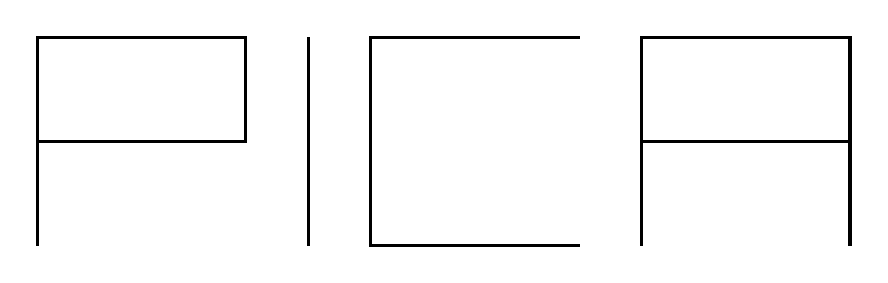
\includegraphics[width=0.9\linewidth]{turtleMPica}
\noindent\hrule\vspace{1.5cm}

In this chapter I describe the creation of robots and the different types of movements that 
robots know about and are capable of performing. I offer some simple experiments for you to 
perform, so that you can practice what you have learned in the previous chapters. I also will 
show you how robots can change direction along the fixed, or \emph{absolute}, points of the compass.


% | caro |
% caro := robot new.
% "letter P"
% caro west; jump: 30 ;jump: 100; north.
% caro go: 100; east; go: 100; south; go: 50.
% caro west; go: 100; south ; jump: 50 ; east.
% caro jump: 130.
% "letter I"
% caro north; go: 100; south; jump: 100; east; jump: 30.
% "letter C" 
% caro jump: 100 ; north;  jump: 100 ; west ; go: 100; 
% south; go: 100; east; go: 100; jump: 30.
% "letter A"
% caro north.
% caro go: 100.
% caro east.
% caro go: 100.
% caro south.
% caro go: 100.
% caro north.
% caro go: 50.
% caro west.
% caro go: 100.



\newpage
\section{Creating Robots}

In the previous chapter you created \emph{a} robot, not \emph{the} robot. That is, robots are not unique, and 
you can create as many robots as you want. Script~\ref{scr:tworobots} creates two robots: pica and daly. 

\begin{script}[tworobots]{Two robots are born.}
| pica daly | 
pica := Bot new. 
daly := Bot new. 
pica color: Color yellow. 
daly jump: 100. 
\end{script}

The second line creates a robot named pica as in Script~\ref{scr:helloworld}. The third line creates a new robot that we refer to using the variable daly. (Just as pica’s name is in homage to Pablo Picasso, that of daly is to honor Salvador Dali.) Both robots are created at the same location on the screen. In line four, we tell pica to change its color to yellow so that we can distinguish the two robots. 

Smalltalk is an object-oriented programming language, as I have mentioned. This means 
not only that we can create objects and interact with them, but that objects can create other 
objects and communicate with them. Moreover, in Smalltalk, there are special objects, called 
classes, that are used to create objects. Sending the message \ct{new} to a class creates an object 
described by its class. Sending the message \ct{new} to the \ct{Bot} class creates a robot. 

To understand what classes are, imagine a class as a sort of factory. A factory for creating 
tin boxes might turn out large numbers of generic boxes, all of the same size, color, and shape. 
After they have been manufactured, some boxes might be filled with biscuits, while others 
might be crushed. When one box is crushed, other boxes are not affected. The same holds for 
objects created inside Squeak. In our case, daly did not change color, but pica did, while pica 
did not move, but daly did. You can think of a class as a factory able to produce unlimited sup- 
plies of objects of the same type. Once produced, each object exists independently of the 
others and can be modified as one wishes. 


In Smalltalk, class names always begin with an uppercase letter. That’s why the name of 
the robot class is \ct{Bot} with an uppercase “B.” Notice that in the command Color yellow, the 
word \ct{Color} is written with an uppercase “C.” That is because \ct{Color} is a class, and what it man- 
ufactures is color objects. By specifying the color name, you get an object of the color you 
want. (The expression \ct{Color yellow} is actually a short form for creating a yellow color object. 
First, a color object is created by sending the message \ct{new} to the class \ct{Color}, and then some 
extra messages define the color to be yellow.) 


\important{A class is a factory that manufactures objects. Sending the message \ct{new} to a class creates an object of that class. Class names always start with an uppercase letter. Here \ct{Bot} is the name of the factory for creating new robots, and \ct{Color} is the factory for colors.

 Thus the command \ct{Bot new color: Color blue} sends a message to the \ct{Bot} class to create a new robot and then sends a message to the new robot to color itself with the color blue.}


\section{Drawing Line Segments}

Asking a robot to draw a line is rather simple, as you already saw in the previous chapter. The message \ct{go: 100} tells a robot to move ahead 100 pixels, and the robot leaves a trace during its move. However, when you draw, even if you are an expert Chinese or Japanese calligrapher, 
you need to lift the brush from time to time. For this purpose, a robot knows how to jump; that 
is, a robot can move without leaving a trace. A robot understands the message \ct{jump:}, whose argument is the same as that for \ct{go:}; namely, it is a distance, given in pixels. Script~\ref{scr:twolines} draws two segments. To keep the picture uncluttered, I have kept the robots out of the illustration 
using the message \ct{beInvisible}. 


\begin{script}[twolines]{Pica is created and then draws two lines.}
!\framebox{
\includegraphics{turtleMTwoLines}}!

| pica | 
pica := Bot new. 
pica go: 30. 
pica jump: 30. 
pica go: 30. 
\end{script}


\begin{experiment}[xp1]{Creating and Moving a Robot}
Experiment by changing the values in the previous script. 
\end{experiment}

\begin{experiment}[sos]{SOS}
Write a script that draws the message "SOS" in Morse code. (In Morse code,an "S" is represented by three short lines, and an "O" is represented by three long lines, as shown in figure below.
 
!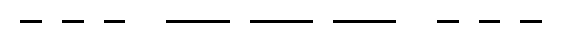
\includegraphics{turtleMSosLines}!
\end{experiment}


\section{Changing Directions}

A robot can orient itself along the eight principal directions of the compass, as shown in 
Figure~\ref{fig:roseDesVents}. The directions are like those on a standard map: \ct{east} is to the right, \ct{west} to the left, \ct{north} up, and \ct{south} down. These directions are absolute, which means that regardless of the  direction in which a robot is currently pointing, if you tell it to point east, the robot will point to the screen’s right, not to the robot’s right. To point a robot in a given absolute direction, just send it a message with the name of the direction. Thus, to tell pica to face south, you simply 
type \ct{pica south}. 

\begin{figure}
\center{\includegraphics[width=10cm]{roseDesVents}}
\caption{The default absolute directions of the compass in which a robot can point. 
\label{fig:roseDesVents}}
\end{figure}

Robots understand the following compass direction messages: \ct{east}, \ct{north}, \ct{northEast}, 
\ct{northWest}, \ct{south}, \ct{southEast}, \ct{southWest}, and \ct{west}. In the next chapter, I will show you how to make a robot turn relative to its current position through an arbitrary angle. 
Script~\ref{scr:gaggle} illustrates the four cardinal directions with four different robots; here Picasso 
and Dali are joined by Paul Klee and Alfred Sisley. Except for pica, who remains in the default 
direction east in which it was created, each robot is oriented in a different direction before 
being told to move. 


\begin{script}[gaggle]{A gaggle of robots go walking.}
| pica daly klee sisl | 
pica := Bot new. 
pica color: Color green. 
pica go: 100. 
daly := Bot new. 
daly north. 
daly color: Color yellow. 
daly go: 100. 
klee := Bot new. 
klee west. 
klee color: Color red. 
klee go: 100. 
sisl := Bot new. 
sisl south. 
sisl go: 100. 
\end{script}

You can use these orientation methods to make more complex drawings. 

\begin{exonofigtitle}{A square}\label{xp:square}
As a first exercise,draw a square with sides of length 50 pixels. Then draw another square of side length 250 pixels. 
\end{exonofigtitle}


\begin{exofigwithsize}[0.5]{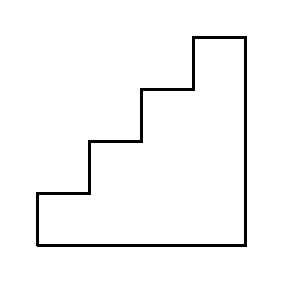
\includegraphics[width=3cm]{turtleMSmallStairs}}{A Staircase}\label{xp:letterA}
You are not limited in your robot drawings to squares. You can create a wide range of geometrical figures.
For example, here is a drawing of a small staircase. Write a script to reproduce this drawing. 
\end{exofigwithsize}


\begin{exofigwithsize}[0.5]{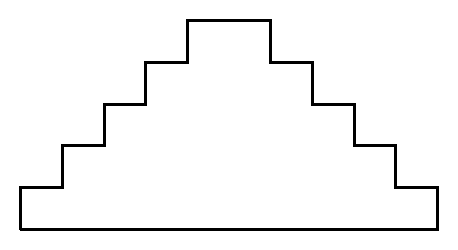
\includegraphics[width=5cm]{turtleMSaqqarah}}{The Step Pyramid of Saqqara}\label{xp:saqq}
Now you are ready to spread your architectural wings and draw a schematic side view of the step pyramid of 
Saqqara,built around 2900 B.C.E. by the architect Imhotep. Write a script to draw a side view of this pyramid, 
as shown in the figure. The pyramid has four terraces,and its top is twice as large as each terrace. 
\end{exofigwithsize}

\begin{exofigwithsize}[0.5]{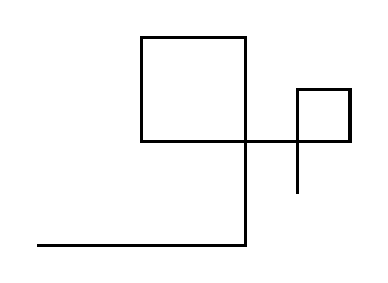
\includegraphics[width=5cm]{turtleMArtNouveau}}{Abstract Art}\label{xp:art}
Write a script to draw the picture shown in the figure below. 
\end{exofigwithsize}


\section{The ABC of Drawing}

Even though you don’t yet have much control over the direction of a robot’s line segments, you 
can start programming pica to write letters. Script~\ref{scr:letterA} draws a rather primitive letter "A." 


% \begin{script}[a]{The letter A is drawn.}
% 	!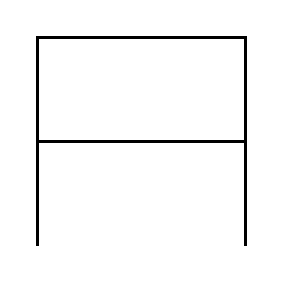
\includegraphics{turtleMLetterA}!
% 	| pica | 
% 	pica := Bot new. 
% 	pica north. 
% 	pica go: 100. 
% 	pica east. 
% 	pica go: 100. 
% 	pica south. 
% 	pica go: 100. 
% 	pica north. 
% 	pica go: 50. 
% 	pica west. 
% 	pica go: 100 
% \end{script}

\begin{scriptfigwithsize}[0.4]{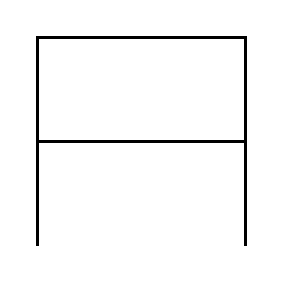
\includegraphics[width=5cm]{turtleMLetterA}}{The letter A}\label{scr:letterA}
	| pica | 
	pica := Bot new. 
	pica north. 
	pica go: 100. 
	pica east. 
	pica go: 100. 
	pica south. 
	pica go: 100. 
	pica north. 
	pica go: 50. 
	pica west. 
	pica go: 100
\end{scriptfigwithsize}




Drawing a letter “C” is no more difficult. You can even write a script to spell out “pica.” 


\begin{exonofigtitle}{Pica}\label{pica}
Draw the name "PICA" as shown at the start of the chapter. To separate the individual letters, you should use the command \ct{jump:}.
\end{exonofigtitle}	
	
	
\note{One could argue that Script 3-4 could be improved. For example,the bottom half of the right- 
hand vertical line of the "A" is drawn twice,since the robot goes back over this segment—once going south, 
once going north—in order to get into position to draw the horizontal bar. Deciding on the best approach to 
solving a programming problem can be a difficult proposition. There are many issues to be considered,such 
as speed,complexity,and readability of the code,and these questions will have different answers depending 
on the programming language and the methods used. However,one approach you might consider is to start 
off by choosing the simplest solution. Then if you are dissatisfied because the program is too slow or doesn’t 
have the particular bells and whistles you want,you can always modify it to speed it up or add other 
enhancements. 
}	
	
	
\section{Controlling Robot Visibility}

You can control whether a robot is to be displayed using the messages \ct{beInvisible} and 
\ct{beVisible}. The message \ct{beInvisible} hides the receiver of the message. A hidden robot acts 
exactly like a normal one; it just doesn’t show where it is. Be careful not to use the method 
\ct{hide}, which is defined by Squeak for its own purposes and can damage the robot environment 
if used improperly. The message \ct{beVisible} makes the robot receiving the message visible. 
A newly created robot is visible by default. 

\section{Summary}

The following table summarizes the expressions and messages encountered in this chapter. 

\noindent
\setlength{\extrarowheight}{1mm}
{\small \begin{tabular}{p{30mm}p{50mm}p{30mm}}
\hline
\textbf{Expressions / Messages}&\textbf{Description}&\textbf{Example}\\\hline
\textsf{Bot new}&Create a robot. &\textsf{pica := Bot new}\\
\textsf{$|$ x y $|$}
&
Declare variables to be used in the \emph{script}
&
\textsf{$|$ pica $|$}
\\
\textsf{jump: {\itshape anInteger}}
&

Tell a robot to move forward a
given number of pixels without 
leaving a trace. 

&
\textsf{pica jump: 10}
\\
\textsf{go: {\itshape unEnter}}
&

Tell a robot to move forward a
given number of pixels while 
leaving a trace. 

&
\textsf{pica go: 10}
\\
\textsf{beInvisible}
&
Diu al robot que s'ha de tornar invisible
&
\textsf{pica beInvisible}
\\
\textsf{beVisible}
&
Diu al robot que s'ha de tornar visible
&
\textsf{pica beVisible}
\\
\textsf{east, northEast, north, northWest, west, southWest, south, southEast.}
&

Tell a robot to point in the
given direction. 

&
\textsf{pica north}
\\
\textsf{Color {\itshape colorName}}
&
Create the color \textit{colorName}
&
\textsf{Color blue}
\\
\textsf{color: {\itshape aColor}}
&
Ask a robot to change its color.
&
\textsf{pica color: Color red}
\\
\hline
\end{tabular}}


	
\ifx\wholebook\relax\else
    \end{document}
\fi

%%% Local Variables:
%%% coding: utf-8
%%% mode: latex
%%% TeX-master: t
%%% TeX-PDF-mode: t
%%% ispell-local-dictionary: "english"
%%% End:
